\section{A dynamical extension of the very simple model}
\label{sec:model}

\subsection{Interaction}

Particles carry fixed discrete color labels
$c\in\{r,g,b,\bar r,\bar g,\bar b\}$ and interact through the
color-weighted, Plummer-softened, screened-Coulomb potential
\begin{equation}
V_{ij}(r) = \frac{C_{ij}}{2}\,\alpha_s\,\hbar c\,
\frac{e^{-r/\lambda_D}}{\sqrt{r^2 + r_0^2}},
\label{eq:potential}
\end{equation}
with no confining term: the system models a deconfined plasma cartoon in
which the string tension is screened, and hadronization proceeds by
capture, not by strings.  The softening $r_0$ plays the role of a quark
wavepacket size and regulates the classical Coulomb collapse; it is a
scanned systematic (Appendix~\ref{app:validation}).

\subsection{Discrete color and the channel prescription}
\label{sec:color-prescription}

The pair factor is the diagonal expectation value of the one-gluon-exchange
operator in the definite-color product state,
$C_{ij}=2\langle c_i c_j|F_1\!\cdot\!F_2|c_i c_j\rangle$, evaluated with the
SU(3) Fierz identity $\sum_a T^a_{ii}T^a_{kk}=\tfrac12(\delta_{ik}-\tfrac13)$:
\begin{equation}
C_{ij} =
\begin{cases}
-2/3 & q\bar q,\ \text{matched}\ (r\bar r):\ \tfrac13\,\mathbf{1}\oplus\tfrac23\,\mathbf{8},\\[2pt]
+1/3 & q\bar q,\ \text{mismatched}\ (r\bar g):\ \mathbf{8},\\[2pt]
+2/3 & qq,\ \text{same}\ (rr):\ \mathbf{6},\\[2pt]
-1/3 & qq,\ \text{different}\ (rg):\ \tfrac12\,\bar{\mathbf 3}\oplus\tfrac12\,\mathbf{6}.
\end{cases}
\label{eq:cij}
\end{equation}
This prescription is the unique energy-conserving choice for fixed labels,
includes the repulsive $\mathbf 6$ and $\mathbf 8$ channels that
Ref.~\cite{Lebed:2016jvq} neglected, and preserves the 2:1
$q\bar q\,{:}\,qq$ attraction ratio, so the $k=\sqrt2$ force criterion
carries over unchanged.  Its counting, however, differs: two thirds of $qq$
pairs are half-strength attractive here, versus Lebed's one third at full
$\bar{\mathbf 3}$ strength (and $3/9$ versus $1/9$ for singlet-content
$q\bar q$).  Appendix~\ref{app:color} quantifies the difference
(a $\sim 9$ percentage-point shift in the static probability at reference
density) and Sec.~\ref{sec:classical-results} treats it as a bracketed
modeling systematic via the \texttt{max\_channel} variant.

\subsection{Flavors and composition}

Flavors $u,d$ ($m=0.34\GeV$), $s$ ($0.48\GeV$) are populated with thermal
Boltzmann weights $n_f \propto m_f^2 T K_2(m_f/T)$ at $T_0$; charm
($1.55\GeV$) is injected as $N_{c\bar c}$ hand-placed pairs mimicking hard
production.  \todo{Table I: full parameter set, defaults, scan ranges.}

\begin{figure}[t]
% 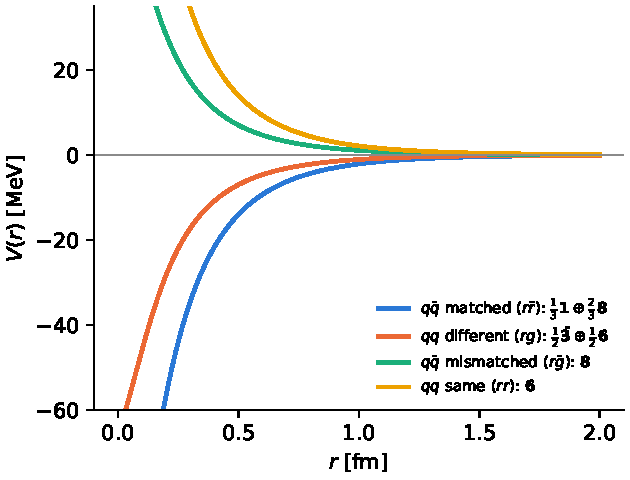
\includegraphics[width=\columnwidth]{figs/fig1_potentials.pdf}
\caption{\todo{Fig.~1: $V(r)$ for the five discrete-color pair classes of
Eq.~\eqref{eq:cij}.}}
\label{fig:potentials}
\end{figure}
